\section{Syndrome weight as an indicator}

From the previous analysis of $\mathcal{A}_{t,\ell}(\mathcal{S})$, the syndrome weights of error vectors causing decoding failures in those sets are low. It is natural to investigate to if the syndrome weight can serve as a predictor for decoding failures. 

For the experiment, for each suitable $r$, we generate $10^3$ instances of non-weak parity check matrices $\mathbf{H}$, random error vectors $e$, and then we compute the average weight of their syndromes $s=He^T$. For decoding failure error vectors, we extract the information from our previous DFR simulations to get the nonweak parity check matrices and the corresponding vector causing decoding failures, and then we compute the average weight of their syndromes. Figure \ref{fig:syndrome-weights} below gives a summary of our results:

\begin{figure}[htbp]
  \begin{center}
    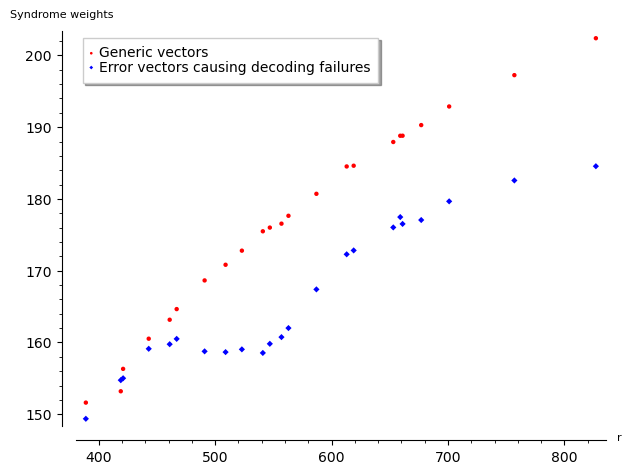
\includegraphics[width=0.49\textwidth]{2_bike/average_sw_generic_vs_DF_T3.png}
    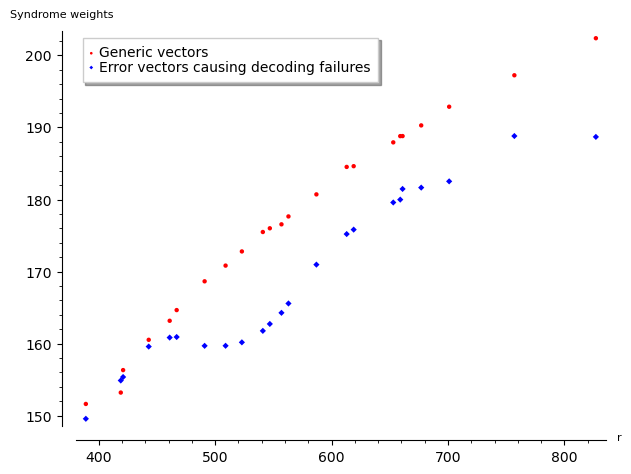
\includegraphics[width=0.49\textwidth]{2_bike/average_sw_generic_vs_DF_random.png}
  \end{center}
  \caption{Distribution of syndrome weights for random error vectors (red) versus error vectors causing decoding failures (blue). The left plot is for non-weak keys (with threshold $T = 3$); the right plot is for unfiltered random keys.}
  \label{fig:syndrome-weights}
\end{figure}

The simulations suggest that syndrome weights of generic vectors tend to follow a normal distribution while the error vectors causing decoding failures have syndrome weights that are more concentrated around the mean, which we hypothesise to be lower than that of the generic vectors; see Figure \ref{fig:r87_comparison} for the case $r=587$, where we compare the syndrome weights of the \todo{check} 128 vectors which caused decoding failures with the syndrome weights of the $10^5$ randomly generated vectors of the same weight $t = 18$.

\todo{might need to generate r587df again}
\begin{figure}[ht]
\centering
\begin{subfigure}[b]{.45\textwidth}
  \centering
  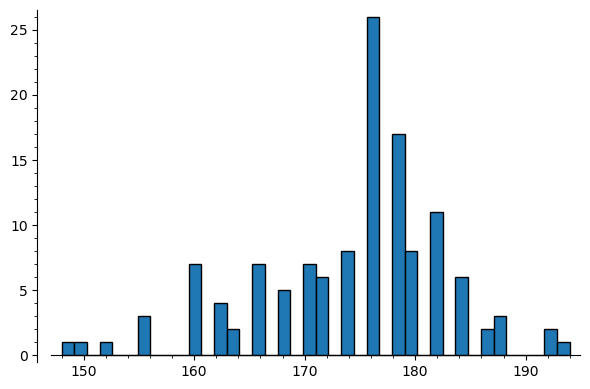
\includegraphics[scale=.45]{2_bike/r587df.png}
  \caption{Decoding failure vectors}
  \label{fig:r587df}
\end{subfigure}
\begin{subfigure}[b]{.45\textwidth}
  \centering
  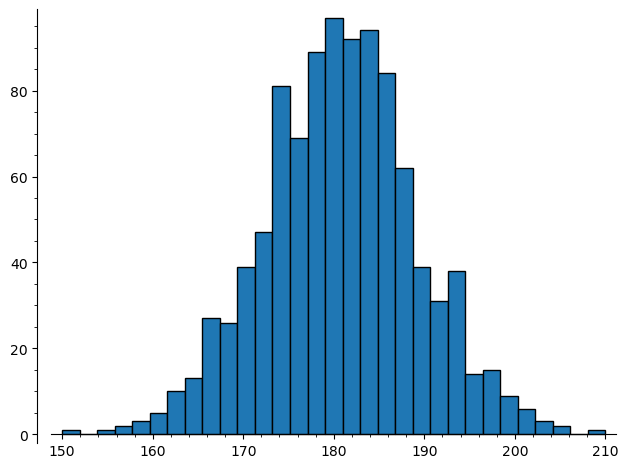
\includegraphics[scale=.45]{2_bike/r587g_new.png}
  \caption{Randomly generated vectors}
  \label{fig:r587g}
\end{subfigure}
\caption{A comparison of syndrome weights for $r = 587$ between the 128 error vectors which were found to be involved in decoding failures and $10^5$ random vectors. Vertical axis is frequency, and horizontal axis is syndrome weight.}
\label{fig:r87_comparison}
\end{figure}

Using this data, we explore whether or not there is convincing evidence that the syndrome weights of error vectors causing decoding failures are lower than those of generic vectors. The null hypothesis is that there is no difference between the two groups in consideration while the alternative hypothesis is that the generic vectors have higher syndrome weights. Both data come from random, independent sampling and have data sets with more than 30 observations. The difference in sample means may be modeled using a $t$-distribution. For each $r$, one could compute the point estimates $m_{\text{generic}} - m_{\text{DF}}$ of population difference $\mu = \mu_{\text{generic}} - \mu_{\text{DF}}$ and standard errors of the point estimate 

$$SE = \sqrt{\frac{\sigma_{\text{generic}}^2}{N_{\text{generic}} } +\frac{\sigma_{\text{DF}}^2}{N_{\text{DF}} } }.$$

With this information, one could compute the test statistic for this (one-tailed) test by the formula $T = \frac{\mu - 0}{SE}$. Using either a $t$-table or statistics software, we can find appropriate degrees of freedom and from there, the $p$-value, for each $r$. Our conclusion is that for the sixteen $r$-values in the range $509 \leq r \leq 827$, the $p$-value is less than the significance value $\alpha = 0.01$, and therefore we reject the null hypothesis, i.e., syndrome weights of error vectors causing decoding failures are lower than those of generic vectors.

A general summary of the test statistic values $m_{\text{generic}} - m_{\text{DF}}$ and the corresponding $p$-values can be found in Table~\ref{table:hyp_test_ts_and_ps}.\todo{check calculations}


\begin{flushleft}
\textbf{Table 6.2}: Hypothesis test results for $509 \leq r \leq 827$, with the corresponding test statistic values and $p$-values, indicating the vectors causing decoding failures do have lower syndrome weights than generic vectors for $509 \leq r \leq 701$, notably a selection of $r$-values where the waterfall region meets the error floor in the DFR graph of Figure~\ref{fig:DFR}.
\end{flushleft}
\begin{table}[ht]\label{table:hyp_test_ts_and_ps}
\centering
\begin{tabular}{c|c|c}
$r$   & $m_{\text{generic}} - m_{\text{DF}}$ & $p$                \\
\hline
509 & 9.29                          & $< 0.00001$ \\
523 & 8.60                          & $< 0.00001$ \\
541 & 9.79                          & $< 0.00001$ \\
547 & 9.29                          & $< 0.00001$ \\
557 & 6.20                          & $< 0.00001$ \\
563 & 8.61                          & $< 0.00001$ \\
587 & 6.56                          & $< 0.00001$ \\
613 & 10.92                         & $< 0.00001$ \\
619 & 8.86                          & $< 0.00001$ \\
653 & 15.99                          & $< 0.00001$ \\
659 & 11.49                          & $< 0.00001$ \\
661 & 9.40                          & $< 0.00001$ \\
677 & 14.45                          & $< 0.00001$ \\
701 & 17.58                          & $< 0.00001$ \\
757 & 16.25                          & $ 0.00278$ \\
827 & 17.53                          & $ 0.00002$ \\

\end{tabular}

\end{table}



